%USE INPUT

\documentclass[12pt]{beamer}
\usepackage[utf8]{inputenc}

\title{Application des machines de Turing aux simulations routières}
\author{Célian Butré}
\date{Session 2022-2023}

\usepackage[T1]{fontenc}       %% gestion de l'encodage (notamment des césure au niveau des caractères accentués)
\usepackage[french]{babel}   %% traitement du texte adapté aux règles typographiques de la langue donnée en option (e.g., pour l'espacement après les ponctuations)
%% Il existe beaucoup de police de caractères à disposition :                               
% \usepackage{times}
% \usepackage{ae}
\usepackage{lmodern}          %% celle-ci est fortement recommandée
%


\usepackage{verbatim}
\usepackage{tikz}
\usepackage{pgfplots}
\usetikzlibrary{arrows, arrows.meta, positioning}

\usepackage{tcolorbox}

\usepackage{graphicx}                  %% pour inclure des figures
\graphicspath{{Images/}}    %%pour inclure les images du fichier images
\usepackage{amsmath, amsthm, amssymb}  %% pour faire de jolies mathématiques, avec plein de symboles supplémentaires
\usepackage{url}                       %% pour inclure des urls (hyperref peut egalement servir, si on veut un lien apparent different du "vrai" lien)
\usepackage{hyperref}                  %% pour les liens (à la fois internes et externes au document)
\usepackage[french,ruled,vlined]{algorithm2e}% pour présenter de jolis algos (il existe aussi le package algorithmics)
%
\usepackage{lastpage}         %% permet de connaître le numéro de la dernière page
%
\usepackage{tikz} %% pour faire des dessins custom
\usetikzlibrary{positioning} %% pour la position relatif

\usetikzlibrary{matrix}




\usepackage{comment} %pour commenter une grande séction facilement

\usepackage{csquotes} %suggéré par le compileur

\newcommand {\monblaze} {\blaze {Célian}{Butré}} %% Pour écrire mon blaze joli
\newcommand {\blaze} [2] {#1 {\sc #2}} %pour écrire un nom très bô
\newcommand{\pourRemplirLesDemandes}[1]{\og #1  \fg}

\newenvironment{uselessNewEnvironment}
{
\begin{center}
\begin{tabular}{|p{5cm}|p{5cm}|p{5cm}|}\hline
}
{
\end{tabular}
\end{center}
}
\usepackage{float} %pour régler un bug?
\pgfplotsset{compat=1.18}


\usetikzlibrary{automata, arrows.meta, positioning}
\usetikzlibrary{overlay-beamer-styles}


\begin{document}


\begin{frame}
  \titlepage
  \begin{center}
      Problématique : «Jusqu'à quel point la machine de Turing est-elle capable de représenter et faire évoluer les
situations routières les plus classiques de la ville ?»
  \end{center}
\end{frame}

\begin{frame}{Plan}
    \tableofcontents
\end{frame}


\section{Préliminaires sur la Machine de Turing}
\subsection{Rappel}
\begin{frame}{Rappel}

\begin{center}

\begin{tikzpicture}
\draw (2,0) -- (2.5,0) -- (2.25,-0.5) -- cycle;
\node at (2.25,-0.20) {\tiny e};
\node at (2.25,-0.15) {};
\end{tikzpicture}



\begin{tabular}{|c|c|c|c|c|c|c|c|c|c|c|c|c|c|c|c|c|c|}\hline
     $\cdot$ & $\cdot$ & $\cdot$ & $\#$ & $\$$ & $s$ & $s$ & $ns$ & $s$ & $a$ & $\$$ & $\$$ & $1$ & $0$ & $0$ & $\cdot$ & $\cdot$ & $\cdot$ \\\hline
     
     
\end{tabular}\\

\vspace{0.5cm}

    $(s,e) \longrightarrow (ns, ne, R)$\\

\begin{tikzpicture}
\draw (2,0) -- (2.5,0) -- (2.25,-0.5) -- cycle;
\node at (2.25,-0.20) {\tiny ne};
\node at (0.5,-0.15) {};
\end{tikzpicture}

\begin{tabular}{|c|c|c|c|c|c|c|c|c|c|c|c|c|c|c|c|c|c|}\hline
     $\cdot$ & $\cdot$ & $\cdot$ & $\#$ & $\$$ & $s$ & $s$ & $ns$ & $ns$ & $a$ & $\$$ & $\$$ & $1$ & $0$ & $0$ & $\cdot$ & $\cdot$ & $\cdot$ \\\hline
     
\end{tabular}
\end{center}
    
\end{frame}

\subsection{Simulateur en C}
\begin{frame}{Préliminaires sur la Machine de Turing}
    
    Simulateur de machines de Turing (en C)
    \newline
    
    
    \begin{itemize}
    \setlength\itemsep{1em}
        \pause
        \item Amélioration Stationnaire (possibilité de rester sur place)
    \end{itemize}
\end{frame}

\subsection{Amélioration Stationnaire}
\begin{frame}{Amélioration Stationnaire}
    \begin{center}
        
    \Large Turing Stationnaire $\Longleftrightarrow$ Turing Classique

    \pause

    \vspace{1cm}

    \Large Turing Stationnaire $\geq$ Turing Classique

    \pause

    \vspace{1cm}

    \Large Turing Stationnaire $\leq$ Turing Classique
    
    \end{center}

    
\end{frame}


\begin{frame}{Turing Stationnaire}
    \begin{center}

\begin{tikzpicture}
\draw (2,0) -- (2.5,0) -- (2.25,-0.5) -- cycle;
\node at (2.25,-0.20) {\tiny e};
\node at (2.9,-0.15) {};
\end{tikzpicture}



\begin{tabular}{|c|c|c|c|c|c|c|c|c|c|c|c|c|c|c|c|c|c|}\hline
     $\cdot$ & $\cdot$ & $\cdot$ & $\cdot$ & $\cdot$ & $\cdot$ & $\cdot$ & $\cdot$ & $s$ & $\cdot$ & $\cdot$ & $\cdot$ & $\cdot$ & $\cdot$ & $\cdot$ & $\cdot$ & $\cdot$ & $\cdot$ \\\hline
     
     
\end{tabular}\\

\vspace{0.5cm}

    $(s,e) \longrightarrow (ns, ne, stationnaire)$\\

\begin{tikzpicture}
\draw (2,0) -- (2.5,0) -- (2.25,-0.5) -- cycle;
\node at (2.25,-0.20) {\tiny ne};
\node at (3.0,-0.15) {};
\end{tikzpicture}

\begin{tabular}{|c|c|c|c|c|c|c|c|c|c|c|c|c|c|c|c|c|c|}\hline
     $\cdot$ & $\cdot$ & $\cdot$ & $\cdot$ & $\cdot$ & $\cdot$ & $\cdot$ & $\cdot$ & $ns$ & $\cdot$ & $\cdot$ & $\cdot$ & $\cdot$ & $\cdot$ & $\cdot$ & $\cdot$ & $\cdot$ & $\cdot$ \\\hline
     
\end{tabular}
\end{center}
\end{frame}
\begin{frame}{Turing Classique}
\begin{center}
    
\begin{tikzpicture}
\draw (2,0) -- (2.5,0) -- (2.25,-0.5) -- cycle;
\node at (2.25,-0.20) {\tiny e};
\node at (2.9,-0.15) {};
\end{tikzpicture}

    \begin{tabular}{|c|c|c|c|c|c|c|c|c|c|c|c|c|c|c|c|c|c|}\hline
     $\cdot$ & $\cdot$ & $\cdot$ & $\cdot$ & $\cdot$ & $\cdot$ & $\cdot$ & $\cdot$ & $s$ & $\$$ & $\cdot$ & $\cdot$ & $\cdot$ & $\cdot$ & $\cdot$ & $\cdot$ & $\cdot$ & $\cdot$ \\\hline    
\end{tabular}\\

        \pause

\vspace{0.5cm}

    $(s,e) \longrightarrow (ns, ne', droite)$\\
    
\begin{tikzpicture}
\draw (2,0) -- (2.5,0) -- (2.25,-0.5) -- cycle;
\node at (2.25,-0.20) {\tiny ne'};
\node at (1.25,-0.15) {};
\end{tikzpicture}

\begin{tabular}{|c|c|c|c|c|c|c|c|c|c|c|c|c|c|c|c|c|c|}\hline
     $\cdot$ & $\cdot$ & $\cdot$ & $\cdot$ & $\cdot$ & $\cdot$ & $\cdot$ & $\cdot$ & $ns$ & $\$$ & $\cdot$ & $\cdot$ & $\cdot$ & $\cdot$ & $\cdot$ & $\cdot$ & $\cdot$ & $\cdot$ \\\hline
     
\end{tabular}\\

        \pause

\vspace{0.5cm}


    $(\$,ne') \longrightarrow (\$, ne, gauche)$\\

\begin{tikzpicture}
\draw (2,0) -- (2.5,0) -- (2.25,-0.5) -- cycle;
\node at (2.25,-0.20) {\tiny ne};
\node at (3,-0.15) {};
\end{tikzpicture}


\begin{tabular}{|c|c|c|c|c|c|c|c|c|c|c|c|c|c|c|c|c|c|}\hline
     $\cdot$ & $\cdot$ & $\cdot$ & $\cdot$ & $\cdot$ & $\cdot$ & $\cdot$ & $\cdot$ & $ns$ & $\$$ & $\cdot$ & $\cdot$ & $\cdot$ & $\cdot$ & $\cdot$ & $\cdot$ & $\cdot$ & $\cdot$ \\\hline
     
\end{tabular}\\

    \end{center}
\end{frame}

\begin{frame}{Amélioration Stationnaire}
\begin{center}
    \begin{tcolorbox}[colframe=red, hbox]
    \large Turing Stationnaire $\Longleftrightarrow$ Turing Classique
\end{tcolorbox}
\end{center}

\end{frame}






\section{Route Unidirectionnelle}
\subsection{Route à vitesse constante}
\begin{frame}{Route à vitesse constante}
\begin{center}
\begin{tikzpicture}
\draw (2,0) -- (2.5,0) -- (2.25,-0.5) -- cycle;
\node at (2.25,-0.20) {\tiny 0};
\node at (9.25,-0.15) {};
\end{tikzpicture}
    \begin{tabular}{|c|c|c|c|c|c|c|c|c|c|c|c|c|c|c|c|c|c|}\hline
     $\cdot$ & $\cdot$ & $\cdot$ & $0$ & $1$ & $1$ & $1$ & $1$ & $0$ & $0$ & $1$ & $1$ & $1$ & $0$ & $0$ & $\cdot$ & $\cdot$ & $\cdot$ \\\hline
     
\end{tabular}\\
\end{center}
\end{frame}

\begin{frame}{Route à vitesse constante}
\begin{center}
\begin{tikzpicture}
\draw (2,0) -- (2.5,0) -- (2.25,-0.5) -- cycle;
\node at (2.25,-0.20) {\tiny 0};
\node at (8,-0.15) {};
\end{tikzpicture}
    \begin{tabular}{|c|c|c|c|c|c|c|c|c|c|c|c|c|c|c|c|c|c|}\hline
     $\cdot$ & $\cdot$ & $\cdot$ & $0$ & $1$ & $1$ & $1$ & $1$ & $0$ & $0$ & $1$ & $1$ & $1$ & $0$ & $0$ & $\cdot$ & $\cdot$ & $\cdot$ \\\hline
     
\end{tabular}\\
\end{center}
\end{frame}

\begin{frame}{Route à vitesse constante}
\begin{center}
\begin{tikzpicture}
\draw (2,0) -- (2.5,0) -- (2.25,-0.5) -- cycle;
\node at (2.25,-0.20) {\tiny 1};
\node at (6.75,-0.15) {};
\end{tikzpicture}
    \begin{tabular}{|c|c|c|c|c|c|c|c|c|c|c|c|c|c|c|c|c|c|}\hline
     $\cdot$ & $\cdot$ & $\cdot$ & $0$ & $0$ & $1$ & $1$ & $1$ & $0$ & $0$ & $1$ & $1$ & $1$ & $0$ & $0$ & $\cdot$ & $\cdot$ & $\cdot$ \\\hline
     
\end{tabular}\\
\end{center}
\end{frame}

\begin{frame}{Route à vitesse constante}
\begin{center}
\begin{tikzpicture}
\draw (2,0) -- (2.5,0) -- (2.25,-0.5) -- cycle;
\node at (2.25,-0.20) {\tiny 1};
\node at (5.5,-0.15) {};
\end{tikzpicture}
    \begin{tabular}{|c|c|c|c|c|c|c|c|c|c|c|c|c|c|c|c|c|c|}\hline
     $\cdot$ & $\cdot$ & $\cdot$ & $0$ & $0$ & $1$ & $1$ & $1$ & $0$ & $0$ & $1$ & $1$ & $1$ & $0$ & $0$ & $\cdot$ & $\cdot$ & $\cdot$ \\\hline
     
\end{tabular}\\
\end{center}
\end{frame}

\begin{frame}{Route à vitesse constante}
\begin{center}
\begin{tikzpicture}
\draw (2,0) -- (2.5,0) -- (2.25,-0.5) -- cycle;
\node at (2.25,-0.20) {\tiny 1};
\node at (4.25,-0.15) {};
\end{tikzpicture}
    \begin{tabular}{|c|c|c|c|c|c|c|c|c|c|c|c|c|c|c|c|c|c|}\hline
     $\cdot$ & $\cdot$ & $\cdot$ & $0$ & $0$ & $1$ & $1$ & $1$ & $0$ & $0$ & $1$ & $1$ & $1$ & $0$ & $0$ & $\cdot$ & $\cdot$ & $\cdot$ \\\hline
     
\end{tabular}\\
\end{center}
\end{frame}

\begin{frame}{Route à vitesse constante}
\begin{center}
\begin{tikzpicture}
\draw (2,0) -- (2.5,0) -- (2.25,-0.5) -- cycle;
\node at (2.25,-0.20) {\tiny 0};
\node at (3,-0.15) {};
\end{tikzpicture}
    \begin{tabular}{|c|c|c|c|c|c|c|c|c|c|c|c|c|c|c|c|c|c|}\hline
     $\cdot$ & $\cdot$ & $\cdot$ & $0$ & $0$ & $1$ & $1$ & $1$ & $1$ & $0$ & $1$ & $1$ & $1$ & $0$ & $0$ & $\cdot$ & $\cdot$ & $\cdot$ \\\hline
     
\end{tabular}\\
\end{center}
\end{frame}

\begin{frame}{Route à vitesse constante}
\begin{center}
\begin{tikzpicture}
\draw (2,0) -- (2.5,0) -- (2.25,-0.5) -- cycle;
\node at (2.25,-0.20) {\tiny 0};
\node at (1.75,-0.15) {};
\end{tikzpicture}
    \begin{tabular}{|c|c|c|c|c|c|c|c|c|c|c|c|c|c|c|c|c|c|}\hline
     $\cdot$ & $\cdot$ & $\cdot$ & $0$ & $0$ & $1$ & $1$ & $1$ & $1$ & $0$ & $1$ & $1$ & $1$ & $0$ & $0$ & $\cdot$ & $\cdot$ & $\cdot$ \\\hline
     
\end{tabular}\\
\end{center}
\end{frame}

\begin{frame}{Route à vitesse constante}
\begin{center}
S'il est possible de prendre ou poser\\
$(1,vide) \longrightarrow (0, plein, droite)$\\
$(0,plein) \longrightarrow (1, vide, droite)$\\

\pause
\vspace{0.5cm}


Sinon\\
$(0,vide) \longrightarrow (0, vide, droite)$\\
$(1,plein) \longrightarrow (1, plein, droite)$\\
\end{center}
\end{frame}

\begin{frame}{Route à vitesse constante}
    \begin{minipage}{\textwidth}
        \begin{center}
            \begin{tikzpicture}
                \draw (2,0) -- (2.5,0) -- (2.25,-0.5) -- cycle;
                \node at (2.25,-0.20) {\tiny 0};
                \node at (-6,-0.15) {};
            \end{tikzpicture}
            \begin{tabular}{|c|c|c|c|c|c|c|c|c|c|c|c|c|c|c|c|c|c|}\hline
                $\cdot$ & $\cdot$ & $\cdot$ & $0$ & $0$ & $1$ & $1$ & $1$ & $1$ & $0$ & $1$ & $1$ & $1$ & $0$ & $0$ & $\cdot$ & $\cdot$ & $\cdot$ \\\hline
            \end{tabular}\\
        \end{center}
        \begin{minipage}{\textwidth}
            \begin{tikzpicture}[overlay]
                \node (a) at (1.375,1.125) {};
                \node (b) at (9.475,1.75) {};
                \draw[->] (b) .. controls (9.5, 2.25) and (1.375,2.25)  .. (a);

            \end{tikzpicture}
        \end{minipage}
    \end{minipage}
\end{frame}

\subsection{Vitesse variable}
\begin{frame}{Vitesse variable}
    \begin{center}
        \begin{tikzpicture}
            \visible<1>{
            \draw[fill=red, draw=black] (0,0) rectangle (0.75,1);
            }
            \draw[fill=red, draw=black] (0.75,0) rectangle (7.5,1);
        
            \node (a) at (0,1) {};
            \node (b) at (7.5,1) {};
            \draw (a) .. controls (0, 3.5) and (3,0.5) .. (3.75,3) .. controls (4.5,0.5) and (7.5,3.5)  .. (b);
            \node at (3.75,3.5) {100 voitures classiques};

            \visible<1>{
            \node (c) at (0,0) {};
            \node (d) at (0.75,0) {};
            \draw (c) .. controls (0, -1.25) and (0.3,0) .. (0.375,-1) .. controls (0.45,0) and (0.75,-1.25)  .. (d);
            \node at (0.375,-1.25) {vitesse};
            }
            \pause
            \pause
            \draw[fill=red, draw=black] (7.5,0) rectangle (8.25, 1);
            \node (c) at (7.5,0) {};
            \node (d) at (8.25,0) {};
            \draw (c) .. controls (7.5, -1.25) and (7.8,0) .. (7.875,-1) .. controls (7.95,0) and (8.25,-1.25)  .. (d);
            \node at (7.875,-1.25) {vitesse};
            
        \end{tikzpicture}
    \end{center}
\end{frame}

\begin{frame}{Vitesse variable}
    \begin{center}
    
        $\text{1 Km/h} \longrightarrow 1$\\
        \vspace{0.5cm}
        $\text{2 Km/h} \longrightarrow 2$\\
        \vspace{0.5cm}
        $\text{3 Km/h} \longrightarrow 3$\\
        \Huge $\vdots$\\
        \Huge $\vdots$\\
        \Huge $\vdots$\\
    \end{center}
\end{frame}

\begin{frame}{Vitesse variable}
    \begin{center}
        \begin{tikzpicture}[node distance = 3cm, on grid, auto,   redstate/.style={state, fill=red!50}]
         
 
            \visible<{1-7,16}>{\node (q0) [state, fill=red!50,fill on=<{1,3,5,6,16}>] {\scriptsize\text{Right}};
            \node (q2) [state, below = of q0, fill=red!50,fill on=<{2,4}>] {\scriptsize\text{Left}};
            
            \path [-stealth, thick]
                (q2) edge [bend left] node[left] {\footnotesize \text{(balise1,balise1,R)}}  (q0)
                (q0) edge [bend left] node[right] {\footnotesize \text{(balise2,balise2,L)}}  (q2)
                (q0) edge [loop left]  node {\footnotesize \text{(0,0,R)}} ()
                (q2) edge [loop right]  node {\footnotesize \text{(\_,\_,L)}}();
            }
            \pause
            \pause
            \pause
            \pause
            \pause

            \visible<6-15>{
            \node (vi1) [state,above left = of q0, fill=red!50,fill on=<{7,8}>] {$v_i$};}
            \visible<6-7>{ 
            \node (vj) [state,above = of q0] {$v_j$};
            \node (vk) [state,above right = of q0] {$v_k$};
            \path [-stealth, thick]
                (q0) edge node[left] {\footnotesize \text{(i,i,S)}}  (vi1)
                (q0) edge node[left] {\footnotesize\text{(j,j,S)}}  (vj)
                (q0) edge node[right] {\footnotesize \text{(k,k,S)}}  (vk);
            }
            
            \pause
            \pause
            \visible<6-15>{
            \node (viR1) [state, right = of vi1, fill=red!50,fill on=<9>] {\scriptsize\text{Right}};
            \node (viL1) [state, right = of viR1, fill=red!50,fill on=<10>] {\scriptsize\text{Left}};

            \node (vi2) [state,below = of vi1, fill=red!50,fill on=<11>] {$v_i$}; 
            \node (viR2) [state, right = of vi2, fill=red!50,fill on=<12>] {\scriptsize\text{Right}};
            \node (viL2) [state, right = of viR2, fill=red!50,fill on=<13>] {\scriptsize\text{Left}};

            \node (vi3) [state,below = of vi2, fill=red!50,fill on=<14>] {$v_i$}; 
            }
            \visible<6-16>{
            \node (viR3) [state, below= of viL2, fill=red!50,fill on=<15>] {\scriptsize\text{Right}};}
            \visible<6-15>{
            \path [-stealth, thick]
                (vi1) edge node[above] {\footnotesize \text{(i,0,R)}}  (viR1)
                (viR1) edge [loop above]  node {\footnotesize \text{(i,i,R)}}()
                (viR1) edge node[above] {\footnotesize\text{(0,i,L)}}  (viL1)
                (viL1) edge [loop above]  node {\footnotesize \text{(i,i,L)}}()
                (viL1) edge node[sloped, above] {\footnotesize \text{(0,0,R)}}  (vi2)
                (vi2) edge node[above] {\footnotesize \text{(i,0,R)}}  (viR2)
                (viR2) edge [loop above]  node [right] {\footnotesize \text{(i,i,R)}}()
                (viR2) edge node[above] {\footnotesize\text{(0,i,L)}}  (viL2)
                (viL2) edge [loop above]  node {\footnotesize \text{(i,i,L)}}();
            \path [dotted, -stealth, thick]
                (viL2) edge node[sloped,above] {\footnotesize \text{i fois}}  (vi3);
            
            \path [-stealth, thick]
                (vi3) edge node[above] {\footnotesize \text{(i,0,R)}}  (viR3)
                (viR3) edge [loop right]  node {\footnotesize \text{(i,i,R)}}();
            }
            \pause
            \pause
            \pause
            \pause
            \pause
            \pause
            \pause
            \pause
            \path [-stealth, thick]
                (viR3) edge [bend right = 50] node[right] {\footnotesize \text{(0,i,R)}}  (q0);
            
        
        \end{tikzpicture}
    \end{center}
\end{frame}

\begin{frame}{Vitesse variable}
    \begin{tikzpicture}
        \node at (0,2.5) {
\includegraphics[width=\textwidth]{Images/Dispersing1.png}};
        \node at (0,0) {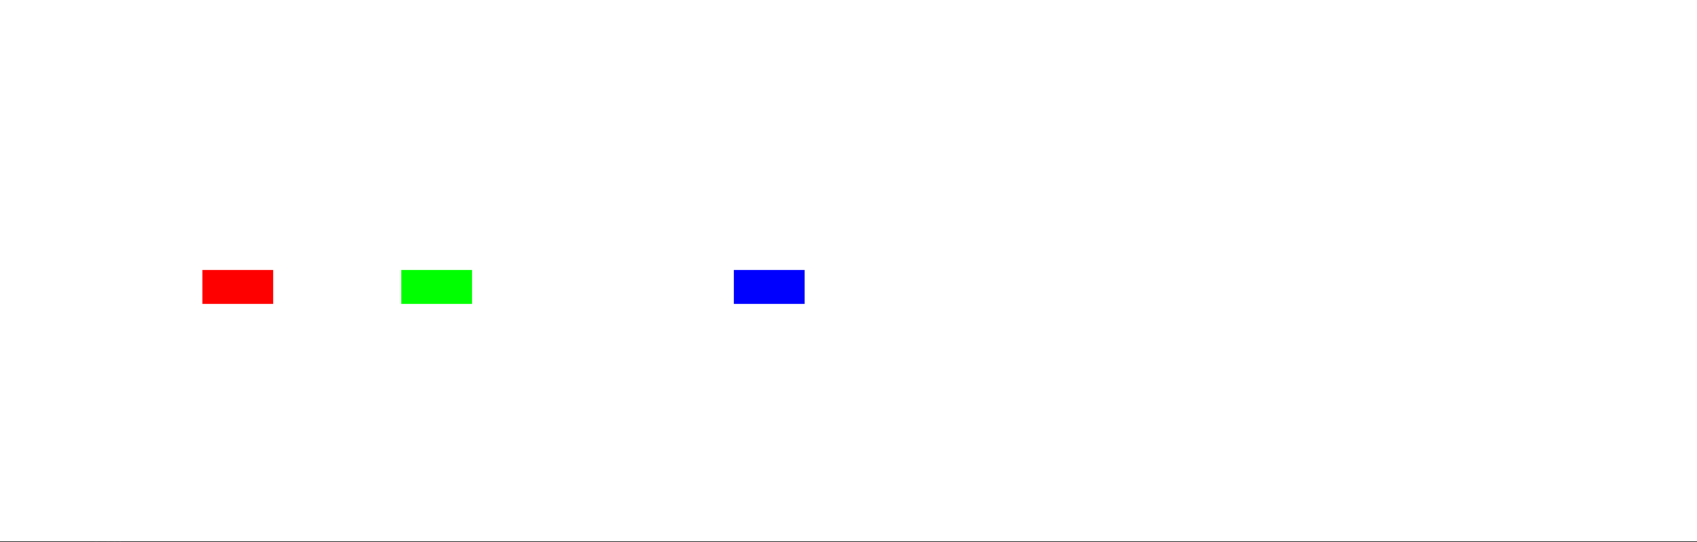
\includegraphics[width=\textwidth]{Images/Dispersing2.png}};
        \node at (0,-2.5) {
\includegraphics[width=\textwidth]{Images/Dispersing3.png}};
    \end{tikzpicture}
\end{frame}

\begin{frame}{Vitesse variable}
    \begin{tikzpicture}
        \node at (0,2.5) {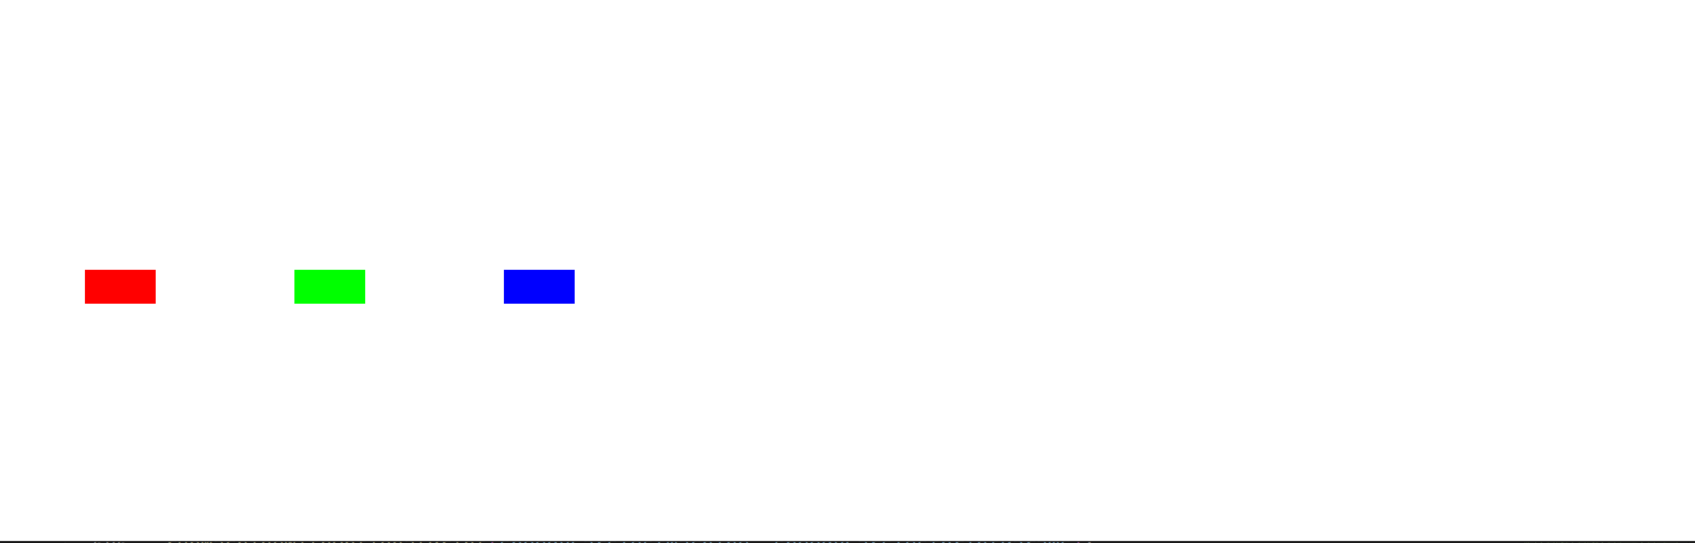
\includegraphics[width=\textwidth]{Images/Crashing1.png}};
        \node at (0,0) {
\includegraphics[width=\textwidth]{Images/Crashing2.png}};
        \node at (0,-2.5) {
\includegraphics[width=\textwidth]{Images/Crashing3.png}};
    \end{tikzpicture}
\end{frame}

\subsection{Freinage}

\begin{frame}{Freinage}
    \begin{center}
        \begin{tikzpicture}

            \node at (2.5, 1.75) {$v_2$};
            \node at (9, 1.75) {$v_1$};
            
            \visible<1>{
            \draw[fill=red, draw=black] (0,0) rectangle (1,1);
            }
            \draw[fill=red, draw=black] (1,0) rectangle (5,1);
            
            \draw (5,1.125) -- (5,1.5) -- (6.5,1.5) -- (6.5, 1.125);
            \node at (5.75,1.75) {E};
            
            \draw (5,-0.125) -- (5,-0.5) -- (6,-0.5) -- (6, -0.125);
            \node at (5.5,-0.75) {Zone de Danger};
            
            \draw[fill=green, draw=black] (6.5,0) rectangle (6.75,1);
            \draw[fill=green, draw=black] (6.75,0) rectangle (11.5,1);

            \visible<2>{
            \draw[fill=red, draw=black] (5,0) rectangle (6,1);
            }
        
        \end{tikzpicture}    
    \end{center}
\end{frame}

\begin{frame}{Freinage}
    \begin{center}
        \begin{tikzpicture}

            \visible<1>{\node at (2.5, 1.75) {$v_2$};}
            \visible<2-3>{\node at (2.5, 1.75) {$v_1$};}
            \node at (9, 1.75) {$v_1$};

            \visible<1>{
            \draw[fill=red, draw=black] (0,0) rectangle (2,1);
            \draw[fill=red, draw=black] (2,0) rectangle (5,1);
            }
            \visible<2-3>{
            \draw[fill=green, draw=black] (0,0) rectangle (0.25,1);
            \draw[fill=green, draw=black] (0.25,0) rectangle (5,1);
            }
            
            \draw (5,1.125) -- (5,1.5) -- (6.5,1.5) -- (6.5, 1.125);
            \node at (5.75,1.75) {E};

            \visible<1>{
            \draw (5,-0.125) -- (5,-0.5) -- (7,-0.5) -- (7, -0.125);
            \node at (6,-0.75) {Zone de Danger};
            }

            \visible<2-3>{
            \draw (5,-0.125) -- (5,-0.5) -- (5.25,-0.5) -- (5.25, -0.125);
            \node at (5.125,-0.75) {Zone de Danger};
            }

            \visible<3>{
            \draw[fill=green, draw=black, opacity = 0.25] (6.25,0) rectangle (6.5,1);
            
            }
            
            \draw[fill=green, draw=black] (6.5,0) rectangle (6.75,1);
            \draw[fill=green, draw=black] (6.75,0) rectangle (11.5,1);
        
        \end{tikzpicture}    
    \end{center}
\end{frame}


\begin{frame}{Freinage}
    \begin{tikzpicture}
        \node at (0,2.5) {
\includegraphics[width=\textwidth]{Images/Slowing1.png}};
        \node at (0,0) {
\includegraphics[width=\textwidth]{Images/Slowing2.png}};
        \node at (0,-2.5) {
\includegraphics[width=\textwidth]{Images/Slowing3.png}};
    \end{tikzpicture}
\end{frame}


\section{Carrefour}

\begin{frame}{Carrefour}
    \begin{center}
           \begin{tikzpicture}
            \foreach \n in {1,1.5,...,5}{
                \draw[draw=black] (0,\n-3) rectangle (0.5,\n-2.5);
            }
            \foreach \n in {1,1.5,...,5}{
                \draw[draw=black] (\n-3,0) rectangle (\n-2.5, 0.5);
            }
            \draw[fill=red, draw=black] (0,0) rectangle (0.5,0.5);
            
            \node at (3.5,0.25) {$=$};

            \foreach \n in {1,1.5,...,5}{
                \draw[draw=black] (\n+3.5,1) rectangle (\n+4, 1.5);
            }
            
            \draw[fill=red, draw=black] (6.5,1) rectangle (7,1.5);
            
            \node at (6.75,0.25) {$+$};
            
            \foreach \n in {1,1.5,...,5}{
                \draw[draw=black] (\n+3.5,-0.5) rectangle (\n+4, -1);
            }
            \draw[fill=red, draw=black] (6.5,-0.5) rectangle (7,-1);
        \end{tikzpicture}
    \end{center}
\end{frame}


\begin{frame}{Carrefour}
    Améliorations nécéssaires
    \begin{itemize}
    \vspace{1cm}
        \item La possibilité de se téléporter
        \vspace{1cm}
        \item Des cases partagées
    \end{itemize}
\end{frame}

\begin{frame}{Carrefour}
    \begin{center}
           \begin{tikzpicture}
            \foreach \n in {1,1.5,...,11}{
                \draw[draw=black] (\n-6,0) rectangle (\n-5.5, 0.5);
            }
            \draw[fill=green, draw=black] (-5,0) rectangle (-4.5,0.5);
            \draw[fill=green, draw=black] (0,0) rectangle (0.5,0.5);
            \draw[fill=green, draw=black] (5,0) rectangle (5.5,0.5);

            \draw[fill=red, draw=black] (-2.5,0) rectangle (-2,0.5);
            \draw[fill=red, draw=black] (2.5,0) rectangle (3,0.5);            
            \end{tikzpicture}
    \end{center}
\end{frame}

\subsection{Amélioration Téléportation}
\begin{frame}{Amélioration Téléportation}
    \begin{center}
    \mbox{\Large Turing Téléportation $\Longleftrightarrow$ Turing Stationnaire}

    \pause

    \vspace{1cm}

    \Large Turing Téléportation $\geq$ Turing Stationnaire

    \pause

    \vspace{1cm}

    \Large Turing Téléportation $\leq$ Turing Stationnaire
    \end{center}
    
\end{frame}

\begin{frame}{Turing Téléportation}
\begin{center}
    
\begin{tikzpicture}
\draw (2,0) -- (2.5,0) -- (2.25,-0.5) -- cycle;
\node at (2.25,-0.20) {\tiny e};
\node at (7.5,-0.15) {};
\end{tikzpicture}

    \begin{tabular}{|c|c|c|c|c|c|c|c|c|c|c|c|c|c|c|c|c|c|}\hline
     $\cdot$ & $\cdot$ & $\cdot$ & $\cdot$ & $B_1s$ & $\$$ & $\$$ & $\$$ & $\$$ & $\$$ & $\$$ & $B_2s$ & $\cdot$ & $\cdot$ & $\cdot$ & $\cdot$ & $\cdot$ & $\cdot$ \\\hline    
\end{tabular}\\

        \pause

\vspace{0.5cm}

    $(B_1s,e) \longrightarrow (B_1ns, ne, B_2)$\\
    
\begin{tikzpicture}
\draw (2,0) -- (2.5,0) -- (2.25,-0.5) -- cycle;
\node at (2.25,-0.20) {\tiny ne};
\node at (-2.5,-0.15) {};
\end{tikzpicture}

\begin{tabular}{|c|c|c|c|c|c|c|c|c|c|c|c|c|c|c|c|c|c|}\hline
     $\cdot$ & $\cdot$ & $\cdot$ & $\cdot$ & $B_1ns$ & $\$$ & $\$$ & $\$$ & $\$$ & $\$$ & $\$$ & $B_2s$ & $\cdot$ & $\cdot$ & $\cdot$ & $\cdot$ & $\cdot$ & $\cdot$ \\\hline    
     
\end{tabular}\\

    \end{center}
\end{frame}

\begin{frame}{Turing Stationnaire}
    \begin{center}
\begin{tikzpicture}
\draw (2,0) -- (2.5,0) -- (2.25,-0.5) -- cycle;
\node at (2.25,-0.20) {\tiny e};
\node at (7.5,-0.15) {};
\end{tikzpicture}

    \begin{tabular}{|c|c|c|c|c|c|c|c|c|c|c|c|c|c|c|c|c|c|}\hline
     $\cdot$ & $\cdot$ & $\cdot$ & $\cdot$ & $B_1s$ & $\$$ & $\$$ & $\$$ & $\$$ & $\$$ & $\$$ & $B_2s$ & $\cdot$ & $\cdot$ & $\cdot$ & $\cdot$ & $\cdot$ & $\cdot$ \\\hline    
\end{tabular}\\

        \pause

\vspace{0.5cm}

    \visible<2>{
    $(B_1s,e) \longrightarrow (B_1ns, ne', R)$\\
}

    \visible<3-8>{
    $(\$,ne') \longrightarrow (\$, ne', R)$\\
}

  
\begin{tikzpicture}
\visible<2>{
\draw (2,0) -- (2.5,0) -- (2.25,-0.5) -- cycle;
\node at (2.25,-0.20) {\tiny ne'};
\node at (1.25,-0.15) {};
}
\visible<3>{
\draw (2.625,0) -- (3.125,0) -- (2.875,-0.5) -- cycle;
\node at (2.875,-0.20) {\tiny ne'};
}
\visible<4>{
\draw (3.25,0) -- (3.75,0) -- (3.5,-0.5) -- cycle;
\node at (3.5,-0.20) {\tiny ne'};
}
\visible<5>{
\draw (3.875,0) -- (4.375,0) -- (4.125,-0.5) -- cycle;
\node at (4.125,-0.20) {\tiny ne'};
}
\visible<6>{
\draw (4.5,0) -- (5,0) -- (4.75,-0.5) -- cycle;
\node at (4.75,-0.20) {\tiny ne'};
}
\visible<7>{
\draw (5.125,0) -- (5.625,0) -- (5.375,-0.5) -- cycle;
\node at (5.375,-0.20) {\tiny ne'};
}
\visible<8>{
\draw (6.125,0) -- (6.625,0) -- (6.375,-0.5) -- cycle;
\node at (6.375,-0.20) {\tiny ne'};
}
\end{tikzpicture}



\begin{tabular}{|c|c|c|c|c|c|c|c|c|c|c|c|c|c|c|c|c|c|}\hline
     $\cdot$ & $\cdot$ & $\cdot$ & $\cdot$ & $B_1ns$ & $\$$ & $\$$ & $\$$ & $\$$ & $\$$ & $\$$ & $B_2s$ & $\cdot$ & $\cdot$ & $\cdot$ & $\cdot$ & $\cdot$ & $\cdot$ \\\hline    
     
\end{tabular}\\

\pause
\pause
\pause
\pause
\pause
\pause

\vspace{0.5cm}

    $(B_2s,ne') \longrightarrow (B_2s, ne, S)$\\


\begin{tikzpicture}
\draw (6.125,0) -- (6.625,0) -- (6.375,-0.5) -- cycle;
\node at (6.375,-0.20) {\tiny ne};
\node at (1.625,-0.15) {};
\end{tikzpicture}

    
\begin{tabular}{|c|c|c|c|c|c|c|c|c|c|c|c|c|c|c|c|c|c|}\hline
     $\cdot$ & $\cdot$ & $\cdot$ & $\cdot$ & $B_1ns$ & $\$$ & $\$$ & $\$$ & $\$$ & $\$$ & $\$$ & $B_2s$ & $\cdot$ & $\cdot$ & $\cdot$ & $\cdot$ & $\cdot$ & $\cdot$ \\\hline    
     
\end{tabular}\\

    \end{center}
\end{frame}

\begin{frame}{Amélioration Téléportation}
\begin{center}
    \begin{tcolorbox}[colframe=red, hbox]
    \large Turing Téléportation $\Longleftrightarrow$ Turing Stationnaire
\end{tcolorbox}
\end{center}

\end{frame}

\subsection{Amélioration Cases Partagées}
\begin{frame}{Amélioration Cases Partagées}
    \begin{center}
    \mbox{\large Turing Cases Partagées $\Longleftrightarrow$ Turing Téléportation}

    \pause

    \vspace{1cm}

    \mbox{\large Turing Cases Partagées $\geq$ Turing Téléportation}

    \pause

    \vspace{1cm}

    \mbox{\large Turing Cases Partagées $\leq$ Turing Téléportation}
    \end{center}
\end{frame}

\begin{frame}{Cases Partagées}
    \begin{center}
    
\begin{tikzpicture}
\draw (2,0) -- (2.5,0) -- (2.25,-0.5) -- cycle;
\node at (2.25,-0.20) {\tiny e};
\node at (7.5,-0.15) {};
\end{tikzpicture}

    \begin{tabular}{|c|c|c|c|c|c|c|c|c|c|c|c|c|c|c|c|c|c|}\hline
     $\cdot$ & $\cdot$ & $\cdot$ & $\cdot$ & $B_1s$ & $\cdot$ & $\cdot$ & $\cdot$ & $\cdot$ & $\cdot$ & $\cdot$ & $B_2s$ & $\cdot$ & $\cdot$ & $\cdot$ & $\cdot$ & $\cdot$ & $\cdot$ \\\hline    
\end{tabular}\\

        \pause

\vspace{0.5cm}

    $(B_1s,e) \longrightarrow (B_1ns, ne, R)$\\
    
\begin{tikzpicture}
\draw (2,0) -- (2.5,0) -- (2.25,-0.5) -- cycle;
\node at (2.25,-0.20) {\tiny ne};
\node at (5.75,-0.15) {};
\end{tikzpicture}

\begin{tabular}{|c|c|c|c|c|c|c|c|c|c|c|c|c|c|c|c|c|c|}\hline
     $\cdot$ & $\cdot$ & $\cdot$ & $\cdot$ & $B_1ns$ & $\cdot$ & $\cdot$ & $\cdot$ & $\cdot$ & $\cdot$ & $\cdot$ & $B_2ns$ & $\cdot$ & $\cdot$ & $\cdot$ & $\cdot$ & $\cdot$ & $\cdot$ \\\hline    
     
\end{tabular}\\

    \end{center}
\end{frame}

\begin{frame}{Turing Téléportation}
    \begin{center}
    
\begin{tikzpicture}
\draw (2,0) -- (2.5,0) -- (2.25,-0.5) -- cycle;
\node at (2.25,-0.20) {\tiny e};
\node at (7.5,-0.15) {};
\end{tikzpicture}

    \begin{tabular}{|c|c|c|c|c|c|c|c|c|c|c|c|c|c|c|c|c|c|}\hline
     $\cdot$ & $\cdot$ & $\cdot$ & $\cdot$ & $B_1s$ & $\cdot$ & $\cdot$ & $\cdot$ & $\cdot$ & $\cdot$ & $\cdot$ & $B_2s$ & $\cdot$ & $\cdot$ & $\cdot$ & $\cdot$ & $\cdot$ & $\cdot$ \\\hline    
\end{tabular}\\

        \pause

\vspace{0.5cm}

    $(B_1s,e) \longrightarrow (B_1ns, ne_1, B_2)$\\
    
\begin{tikzpicture}
\draw (2,0) -- (2.5,0) -- (2.25,-0.5) -- cycle;
\node at (2.25,-0.20) {\tiny ne$_1$};
\node at (-1.5,-0.15) {};
\end{tikzpicture}

\begin{tabular}{|c|c|c|c|c|c|c|c|c|c|c|c|c|c|c|c|c|c|}\hline
     $\cdot$ & $\cdot$ & $\cdot$ & $\cdot$ & $B_1ns$ & $\cdot$ & $\cdot$ & $\cdot$ & $\cdot$ & $\cdot$ & $\cdot$ & $B_2s$ & $\cdot$ & $\cdot$ & $\cdot$ & $\cdot$ & $\cdot$ & $\cdot$ \\\hline    
     
\end{tabular}\\

        \pause

\vspace{0.5cm}

    $(B_2s,ne_1) \longrightarrow (B_2ns, ne_2, B_1)$\\
    
\begin{tikzpicture}
\draw (2,0) -- (2.5,0) -- (2.25,-0.5) -- cycle;
\node at (2.25,-0.20) {\tiny ne$_2$};
\node at (7.5,-0.15) {};
\end{tikzpicture}

\begin{tabular}{|c|c|c|c|c|c|c|c|c|c|c|c|c|c|c|c|c|c|}\hline
     $\cdot$ & $\cdot$ & $\cdot$ & $\cdot$ & $B_1ns$ & $\cdot$ & $\cdot$ & $\cdot$ & $\cdot$ & $\cdot$ & $\cdot$ & $B_2ns$ & $\cdot$ & $\cdot$ & $\cdot$ & $\cdot$ & $\cdot$ & $\cdot$ \\\hline    
     
\end{tabular}\\

        \pause

\vspace{0.5cm}

    $(B_1ns,ne_2) \longrightarrow (B_1ns, ne, R)$\\
    
\begin{tikzpicture}
\draw (2,0) -- (2.5,0) -- (2.25,-0.5) -- cycle;
\node at (2.25,-0.20) {\tiny ne};
\node at (5.75,-0.15) {};
\end{tikzpicture}

\begin{tabular}{|c|c|c|c|c|c|c|c|c|c|c|c|c|c|c|c|c|c|}\hline
     $\cdot$ & $\cdot$ & $\cdot$ & $\cdot$ & $B_1ns$ & $\cdot$ & $\cdot$ & $\cdot$ & $\cdot$ & $\cdot$ & $\cdot$ & $B_2ns$ & $\cdot$ & $\cdot$ & $\cdot$ & $\cdot$ & $\cdot$ & $\cdot$ \\\hline    
     
\end{tabular}\\

    \end{center}
\end{frame}

\begin{frame}{Amélioration Cases Partagées}
\begin{center}
    \begin{tcolorbox}[colframe=red, hbox]
    \large Turing Cases Partagées $\Longleftrightarrow$ Turing Téléportation
\end{tcolorbox}
\end{center}

\end{frame}

\subsection{Simulation Carrefour}
\begin{frame}{Simulation Carrefour}
    Symboles
    \begin{itemize}
    \vspace{1cm}
        \item Vide $\longrightarrow$ 0 \visible<2>{(4 au centre)}\\
        \vspace{1cm}
        \item Voiture horizontale $\longrightarrow$ 7 \visible<2>{(5 au centre)}\\
        \vspace{1cm}
        \item Voiture verticale $\longrightarrow$ 8 \visible<2>{(6 au centre)}\\
    \end{itemize}
\end{frame}

\begin{frame}{Simulation Carrefour}
    \begin{enumerate}
        \item Déplacer les voitures horizontales, en amont
        \item Cases Partagées
        \item Déplacer les voitures horizontales, en aval
        \item Téléportation
        \item Déplacer les voitures verticales, en amont
        \item Cases Partagées
        \item Déplacer les voitures verticales, en aval
        \item Téléportation
    \end{enumerate}
\end{frame}

\begin{frame}{Simulation Carrefour}
\begin{enumerate}
    \setcounter{enumi}{0}
    \visible<1-7>{\item Déplacer les voitures horizontales, en amont}
    \setcounter{enumi}{2}
    \visible<8>{\item Déplacer les voitures horizontales, en aval}
    \setcounter{enumi}{4}
    \visible<1-7>{\item Déplacer les voitures verticales, en amont}
    \setcounter{enumi}{6}
    \visible<8>{\item Déplacer les voitures verticales, en aval}
\end{enumerate}

\begin{tikzpicture}
    
\foreach \n in {1,2,...,3}{
            \draw[draw=black] (0,\n-2) rectangle (1,\n-1);
            }
            \foreach \n in {1,2,...,6}{
                \draw[draw=black] (\n-5,0) rectangle (\n-4, 1);
            }
            \draw[fill=red, draw=black] (0,-1) rectangle (1,0);
            \draw[fill=red, draw=black] (0,0) rectangle (1,1);
            \draw[fill=red, draw=black] (0,1) rectangle (1,2);

            \visible<{1,7-8}>{\draw[fill=green, draw=black] (-3,0) rectangle (-2,1);}
            \draw[fill=green, draw=black] (-2,0) rectangle (-1,1);
            \draw[fill=green, draw=black] (-1,0) rectangle (0,1);

            \visible<{1,7}>{\draw[->] (-2.5,2) -- (-2.5,1);}
            \visible<{2,6}>{\draw[->] (-1.5,2) -- (-1.5,1);}
            \visible<{3,5}>{\draw[->] (-0.5,2) -- (-0.5,1);}
            \visible<4>{\draw[->] (-1,2) -- (0,1);}
            \visible<8>{\draw[->] (1.5,2) -- (1.5,1);}
            


\end{tikzpicture}
            
\end{frame}

\begin{frame}{Simulation Carrefour}
    \begin{tikzpicture}
        \node at (0,2.5) {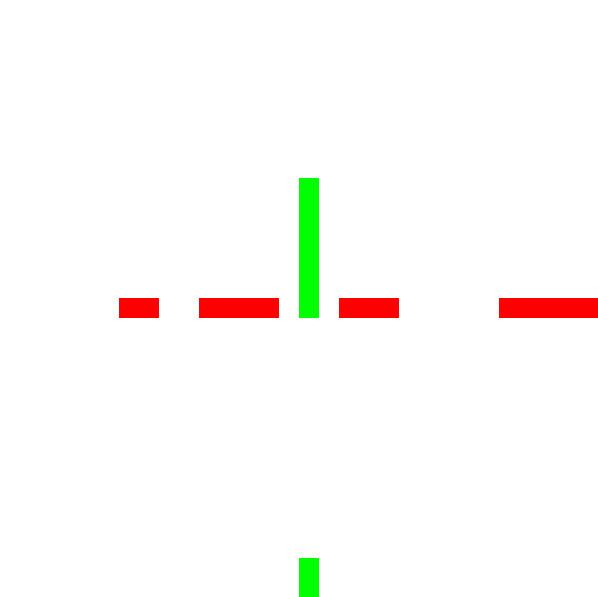
\includegraphics[width=4cm]{Images/Carrefour1.png}};
        \node at (0,0) {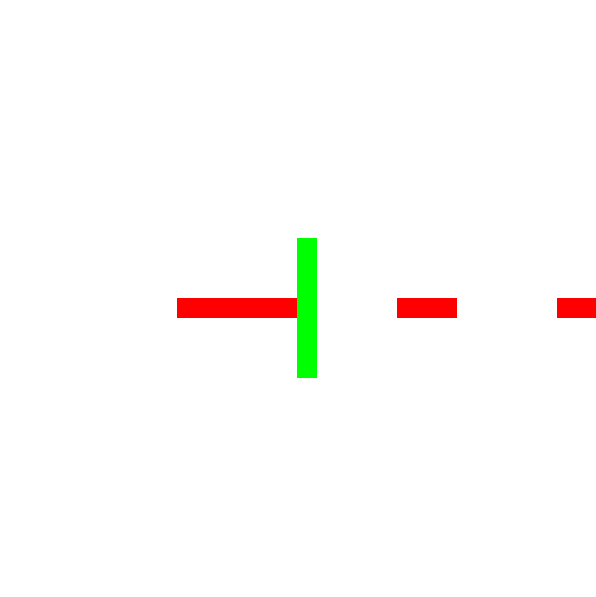
\includegraphics[width=4cm]{Images/Carrefour2.png}};
        \node at (0,-2.5) {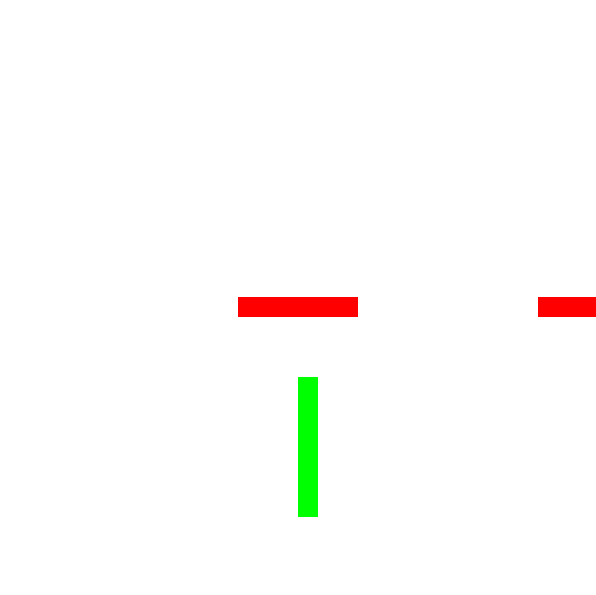
\includegraphics[width=4cm]{Images/Carrefour3.png}};
    \end{tikzpicture}
\end{frame}

\section{Limites du modèle}
\begin{frame}{Limites du modèle}
\begin{center}
    \begin{tabular}{|c|c|c|}
    \hline
     & Route Simple & Carrefour Simple \\
    \hline
    Symboles & \visible<2-4>{3} & \visible<2-4>{9} \\
    \hline
    États & \visible<3-4>{3} & \visible<3-4>{23} \\
    \hline
    Transitions & \visible<4>{6} & \visible<4>{89} \\
    \hline
    
\end{tabular}

\end{center}

\end{frame}

\section{Conclusion}
\begin{frame}{Conclusion}
    \begin{center}
        \begin{align*}
            \visible<2-6>{\text{Machine de Turing} &= \text{Théorique}\\}
            \visible<3-6>{\text{Équivalences} &= \text{Intéressant} \\}
            \visible<4-6>{\text{Petite Échelle} &= \text{Ludique}\\}
            \visible<5-6>{\text{Grande Échelle} &= \text{Difficile}\\}
            \visible<6>{\text{Acquis} &= \text{Revues}\\}
        \end{align*}
    \end{center}
\end{frame}
\end{document}
